\chapter{Coherent Light and Single Photons}
\label{sec:5_coherent_light_single_photons}

In this chapter, we will look at why light is such an integral part of modern day communication.
We will discuss the difference between coherent and incoherent light, and outline the basic principle behind producing coherent light using lasers.
Finally, we will transition to talking about light in the context of quantum communication that relies on single photons as information carriers.

\section{Introduction}
\label{sec:5-1_intoduction}

Why do we want to encode information as optical signals?
Light is a very good carrier of information because it is incredibly \textit{\textbf{fast}}.
Table~\ref{tab:5-1_speed_light} summarizes the speed of light in various media.
\begin{table}[b!]
    \centering
    \begin{tabular}{c|c|c}
        vacuum & $c$ & $2.998\times10^{8} \; \text{ms}^{-1}$  \\
        \hline
        air & $c/1.0003$ & $2.998\times10^{8} \; \text{ms}^{-1}$  \\
        \hline
        silica fiber & $c/1.47$ & $2.039\times10^{8} \; \text{ms}^{-1}$
    \end{tabular}
    \caption[Speed of light]{Speed of light in various media.}
    \label{tab:5-1_speed_light}
\end{table}
In vacuum, the speed of light is $c=2.998\times 10^8$ $\text{ms}^{-1}$.
Here on Earth, most of the time we do not send light through vacuum.
However, even in air the light slows by only the small factor of 1.0003.
Most often, we use fiber optic cables made from pure silica glass with refractive index of 1.47.
This decreases the speed of light somewhat but still remains very fast.

Apart from being fast, light is also relatively \textit{\textbf{easy to produce}}.
Even in the early days of civilization, a reliable source of light was fire.
We saw an example of this when we learnt about optical telegraphy used for rapid communication on the Great Wall of China in Chapter~\ref{sec:1_Introduction}.
Today, we mainly use lasers and send the optical signals through fibers.
Due to their ability to produce highly coherent light, lasers had a transformative impact not only on the way we communicate but on many other aspects of our lives. 

The third reason why light is so useful in communication is that photons do not interact easily with each other.
Once in flight, photons will continue speeding to their destination nearly unaffected.
This makes optical signals \textit{\textbf{robust to noise}}.
Compare this with copper wires carrying electric signals.
The moving electrons are susceptible to external electric and magnetic noise and require thorough shielding to protect the integrity of the signal.
Furthermore, the moving electrons themselves produce electromagnetic fields which may affect other nearby carriers of electric signals.
This means that copper wires cannot be packed too closely to each other.
In contrast, this is not the case for optical fibers.

\begin{figure}[t]
    \centering
    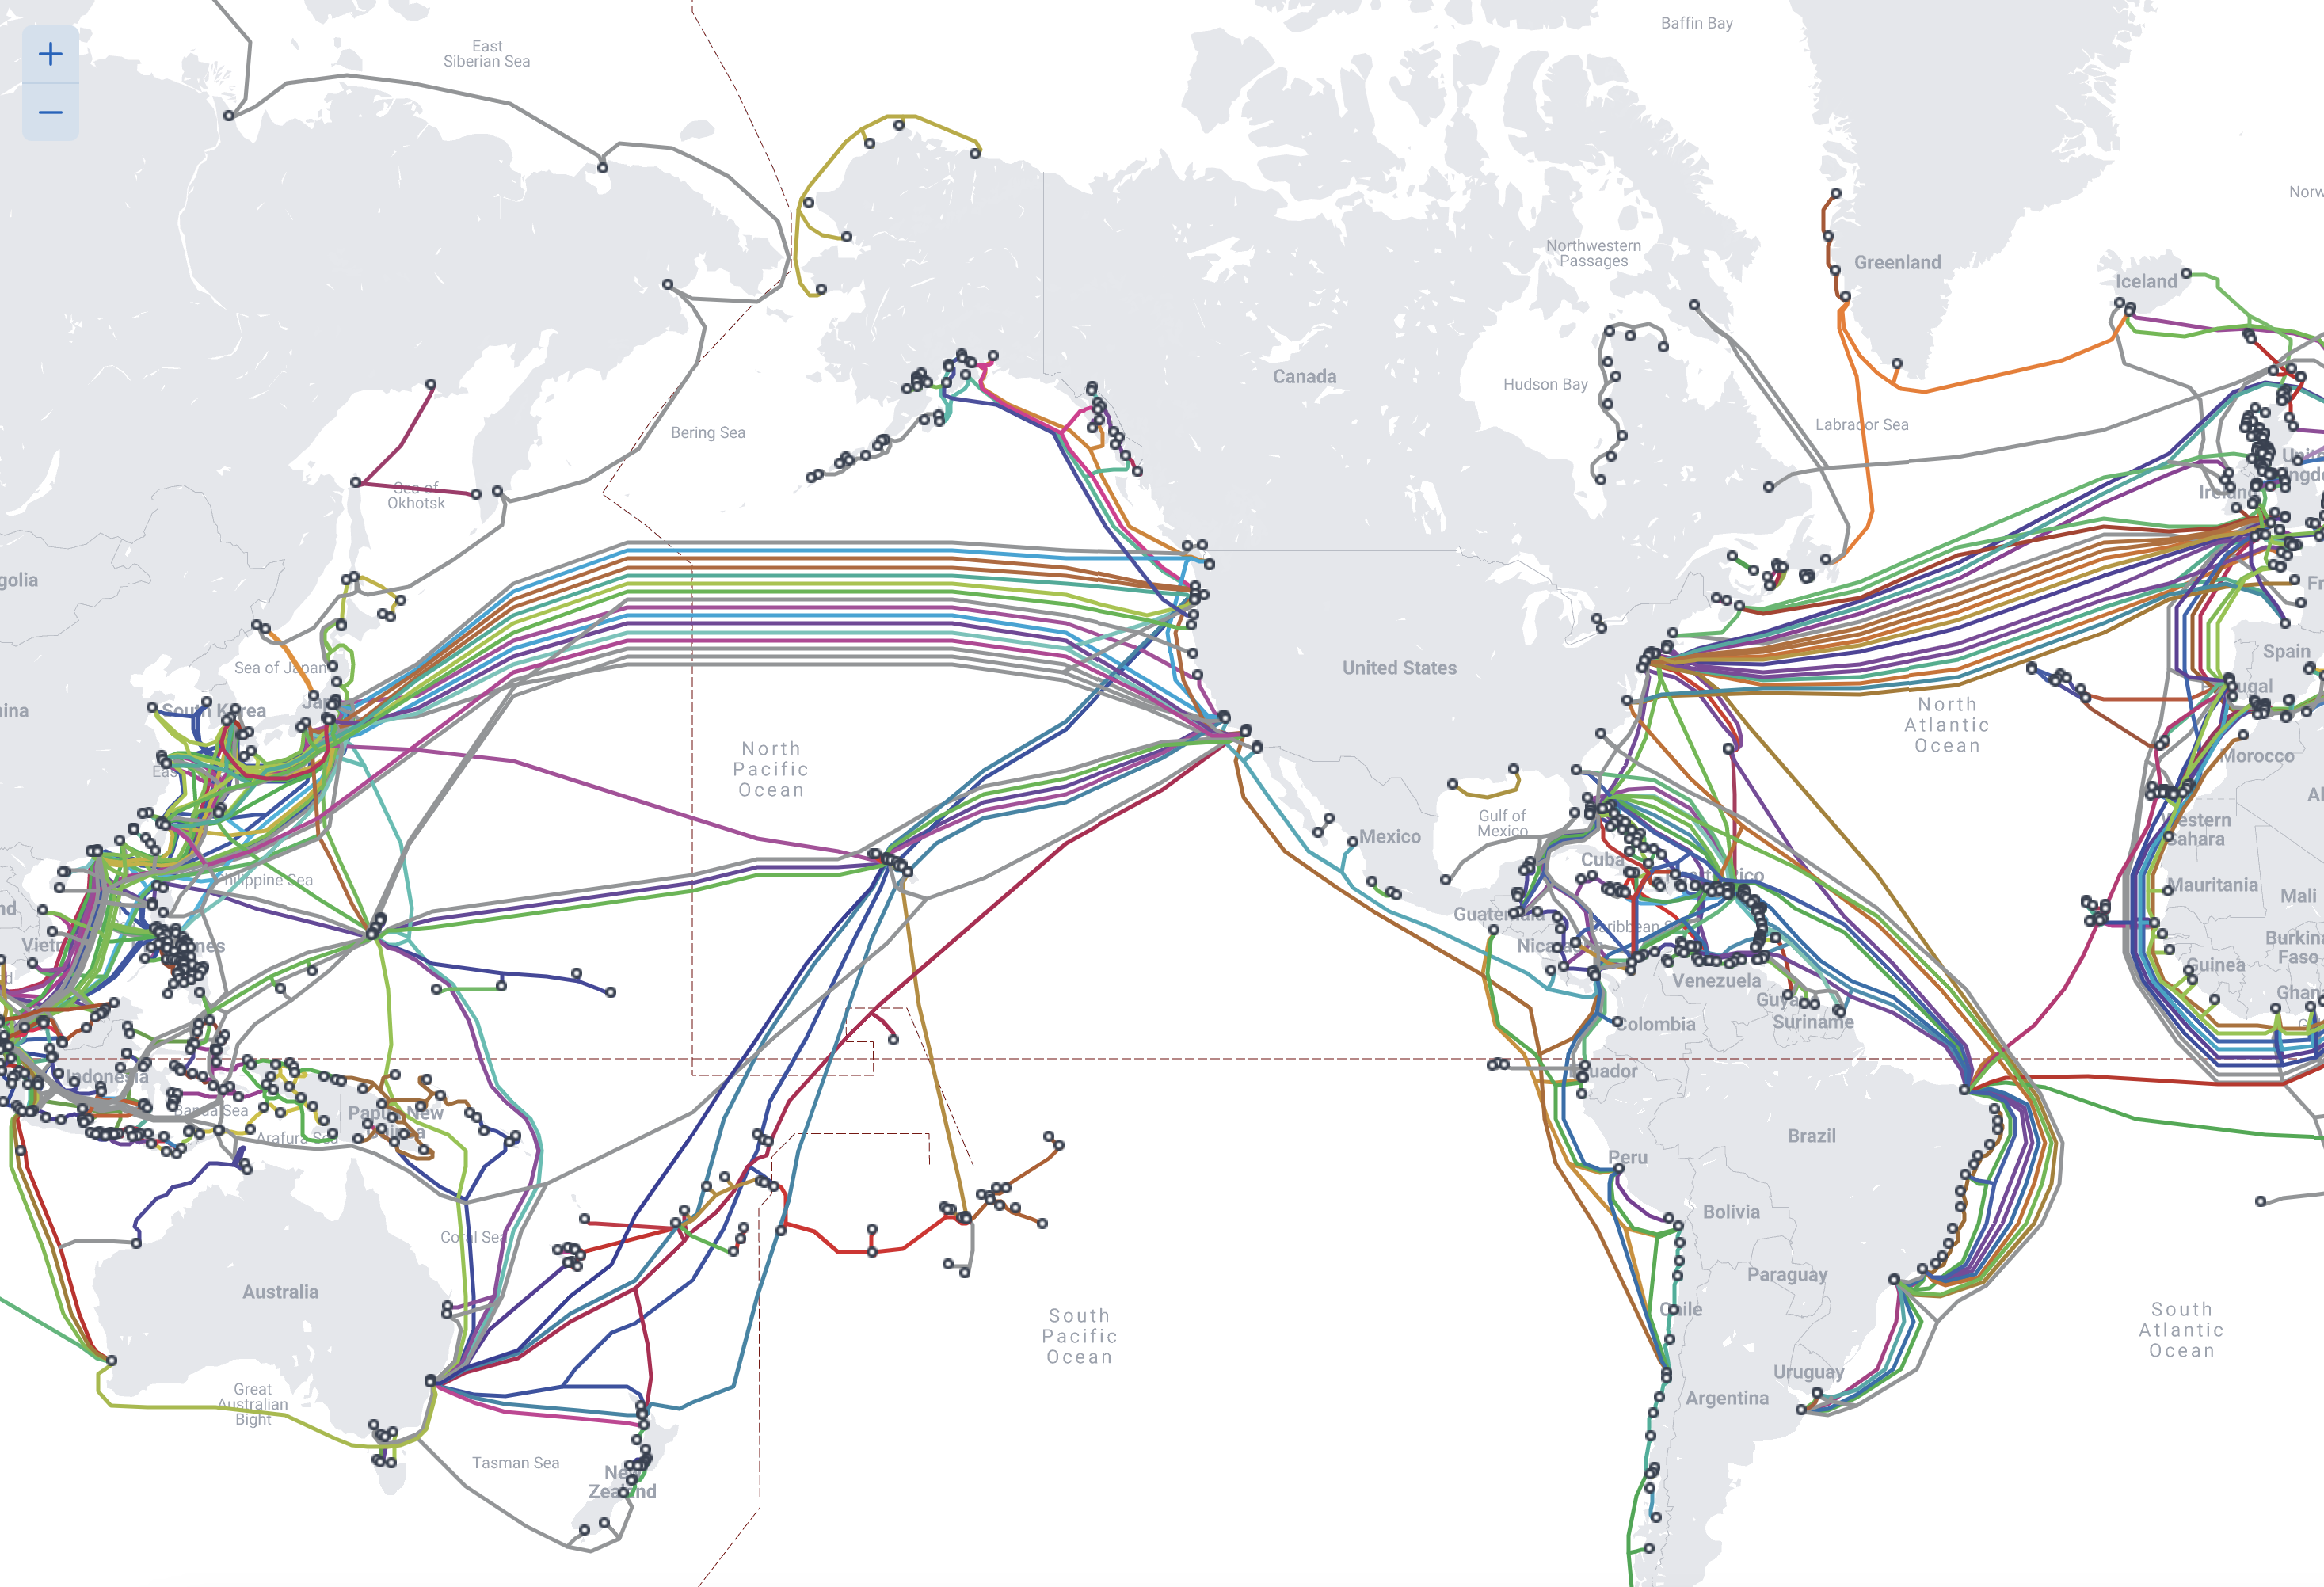
\includegraphics[width=0.8\textwidth]{lesson5/5-1_underwater_cable_map.png}
    \caption[Underwater cabel map]{Map of submarine cables.}
    \label{fig:5-1_underwater_cable_map}
\end{figure}

Optics has always played an important role in communication.
We saw a couple of examples of that already in the Great Wall of China and Napoleon's semaphore in chapter~\ref{sec:1_Introduction}.
These methods were limited in the sense that you had to have a direct visual path between the sender and the receiver, you needed good weather conditions, and in the case of Napoleon's semaphore, it only worked during the day.
\textit{\textbf{Waveguides}} circumvent all these problems.
Use of electric wires and optical fibers sparked a rapid expansion in our ability to communicate fast and far.
Figure~\ref{fig:5-1_underwater_cable_map} shows a map of submarine cables \footnote{This map was obtained from TeleGeography at \href{https://www.submarinecablemap.com/}{https://www.submarinecablemap.com/} under the \href{https://creativecommons.org/licenses/by-sa/4.0/}{CC BY-SA 4.0} license.}, connecting the continents.
It is these cables that allow seamless global communication at incredible speeds.

In this chapter, we are going to be concerned with how to produce three types of light.
We will begin with \textit{\textbf{incoherent light}}\index{incoherent light}.
This is light that can be produced by burning fuel or heating a gas.
We will explain in what sense this light is incoherent and what it means in Section~\ref{sec:5-2_coherent_vs_incoherent}.
Incoherent light is very easy to produce, which is why it played an important historical role as we have discussed already.
This type of light is known as a classical state of light as it does not manifest any quantum behavior.

We will compare incoherent light with \textit{\textbf{coherent light}}\index{coherent light} produced by lasers. The main mechanism behind producing this light is known as stimulated emission, which we will discuss in Sec.~\ref{sec:5-3_lasers1} and Sec.~\ref{sec:5-4_lasers2}.
Lasers sparked the first information revolution and therefore play an important historical role.
Despite its coherent nature, light produced by lasers is still not fully quantum. 
Developments in laser technology over the last decades have led to great proliferation of available sources of coherent light.
Lasers range from large and powerful ones found in high-tech laboratories to small pointer devices hanging from our keychains.

We will conclude this chapter by looking at \textit{\textbf{single photon sources}} in Sec~\ref{sec:5-5_single_photons}.
We will discuss three ways to produce single photons.
The first one is by attenuation of laser light.
The second method is by using heralded photons.
The third way is to use genuine emitters of single photons, such as nitrogen vacancy centres in diamond.
Compared to the previous two types of light, single photons are very difficult to make.
They can be only produced in laboratories or devices that meet very stringent requirements, but they can display quantum behavior, which is why they are crucial in quantum communication.


\section{Coherent vs incoherent light}
\label{sec:5-2_coherent_vs_incoherent}

\begin{figure}
    \centering
    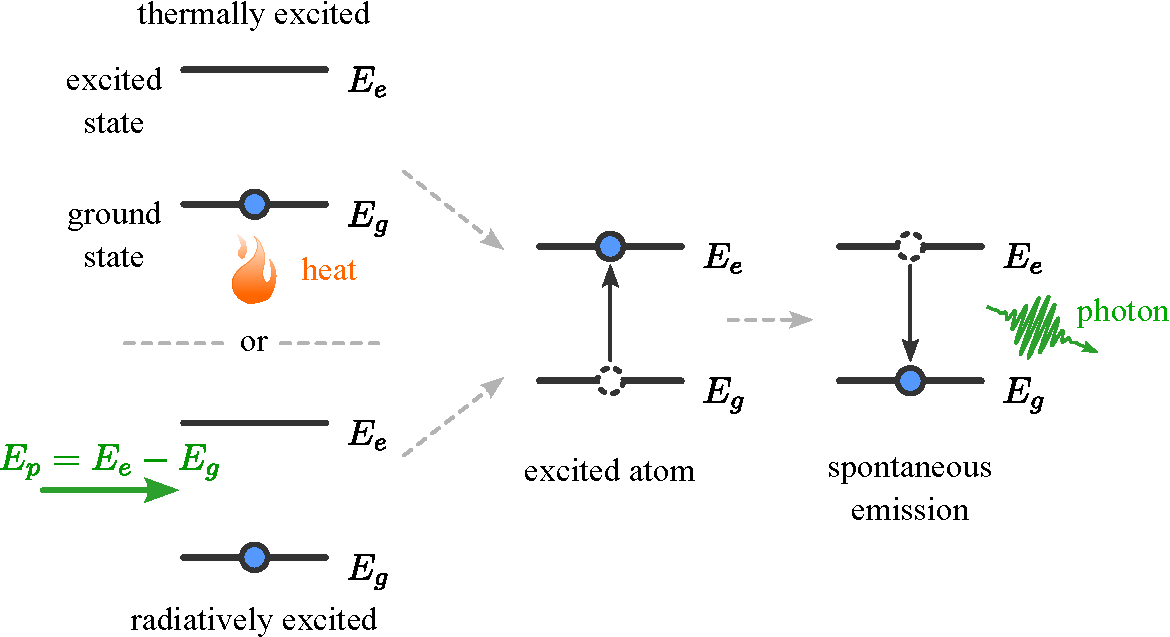
\includegraphics[width=\textwidth]{lesson5/5-2_spontaneous_emission.pdf}
    \caption[Spontaneous emission]{A two-level atom is excited either thermally or radiatively. After some time it deexcites via spontaneous emission producing a photon of light.}
    \label{fig:5-2_spontaneous_emission}
\end{figure}

How does matter radiate light?
Let's consider a model of a simple two-level atom as shown in Fig.~\ref{fig:5-2_spontaneous_emission}.
The ground state has energy $E_g$ and the excited state has energy $E_e$.
The state of the atom is pictured by the blue circle.
In order to produce light, the atom needs to first receive energy.
One way to do that is through heat.
If this is the case, we say the atom becomes \textit{\textbf{thermally excited}}.
Another way is to excite the atom with radiation.
A different way of exciting the atom is to irradiate it with light of the right energy.
The atom can absorb radiation of energy equal to the difference of energies between the excited and ground states, $E_p = E_e - E_g$.
When this happens, we say the atom has been \textit{\textbf{radiatively excited}}.
After some time, the atom releases the stored energy in the form of a photon of light.
This process happens without an external stimulus at a random time and is called \textit{\textbf{spontaneous emission}}.

Let's consider two such excited atoms as shown in Fig.~\ref{fig:5-2_incoherent_emission}.
After some time, both atoms undergo the process of spontaneous emission producing one photon each.
The direction of emission is random and therefore different for both atoms.
Furthermore, both photons have random and different phases.
We call such light to be incoherent.

We can go one step further and consider a large number of atoms emitting light.
To be more specific, we can consider an incandescent light bulb.
Here, a filament is heated up by an electric current running through it.
This in turn excites the atoms in the filament which eventually undergo spontaneous emission producing a large amount of photons.
Not only are these photons travelling in all possible directions and are out to phase, their energies are different as well.
This is because the atoms in the filament have a much more complicated energy level structure than our simple two-level model.
In conclusion, incoherent light is composed of components with different energies travelling in different directions, each having a different phase.

\begin{figure}
    \centering
    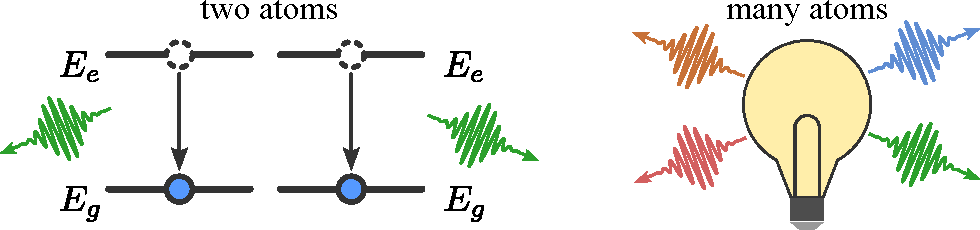
\includegraphics[width=0.8\textwidth]{lesson5/5-2_incoherent_emission.pdf}
    \caption[Incoherent emission]{Two or more atoms emitting incoherently.}
    \label{fig:5-2_incoherent_emission}
\end{figure}

The question that you might be asking yourself is, what does it take to produce light?
% the opposite is true.
How can we make light that has a single component of the same energy, travelling in the same direction and with the same phase?
We will answer this question in the next two sections.



\section{Lasers I: Stimulated emission}
\label{sec:5-3_lasers1}

%Step three: lasers, one.

In this section, we address the question that was raised at the end of the previous section.
What are the basic ingredients to make coherent light.
Such light is in-phase, monochromatic and travels in the same direction.
Typical example of a source that produces light with these properties is the \textit{\textbf{laser}}.
Laser stands for ``light amplification via stimulated emission of radiation''.
Let's have a look at what these individual words mean.

We begin with \textit{\textbf{stimulated emission}}, which is the physical process behind lasing.
We have encountered two of the three fundamental ways in which light interacts with matter, namely stimulated absorption and spontaneous emission, also shown in Fig.~\ref{fig:5-3_light_matter_interaction}.
Stimulated absorption is when an atom, initially in the ground state interacts with an incoming photon. If the frequency of the photon is just right, the atom may absorb this photon, and the atom becomes excited.
Spontaneous emission is when an initially excited atom emits a photon of light without any external stimulus.
Stimulated emission on the other hand is when an initially excited atom interacts with an incoming photon.
This causes the atom to emit a photon of light.
But this time, the emitted photon of light has the same energy as the external photon, same phase and crucially it is emitted in the same direction.
In other words, the two photons are coherent, and it is through the process of stimulated emission that coherent light can be produced.

\begin{figure}[t]
    \centering
    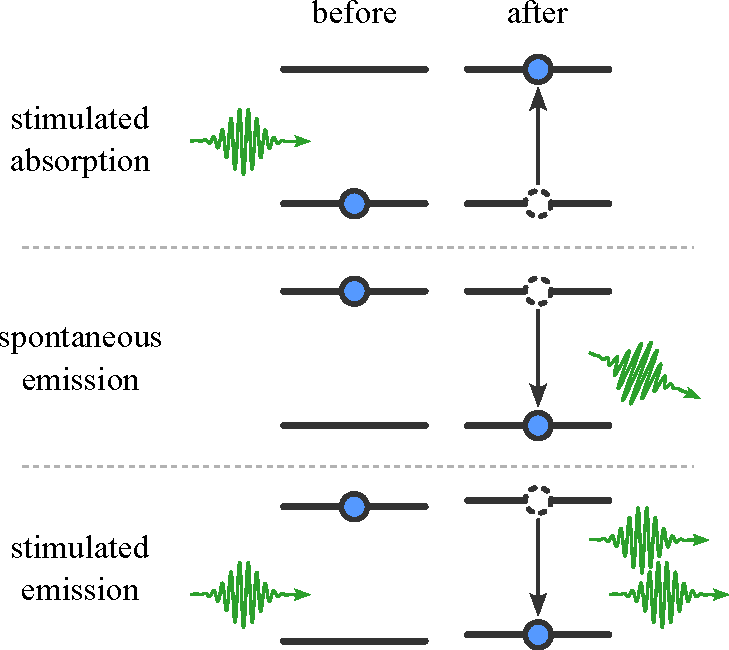
\includegraphics[width=0.55\textwidth]{lesson5/5-3_three_interactions.pdf}
    \caption[Light-matter interactions]{Three fundamental types of light-matter interactions.}
    \label{fig:5-3_light_matter_interaction}
\end{figure}

We can see from Fig.~\ref{fig:5-3_light_matter_interaction} that stimulated emission starts with a single photon and finishes with two coherent photons.
This opens up the possibility of amplifying light, which brings us to the ``light amplification'' part of the laser.
Imagine having a large number of atoms in the excited state.
A single photon of light can stimulate the first atom to emit a photon.
Both photons (the initial one and the newly emitted one) can now stimulate further atoms to emit triggering an cascade of emissions and producing a coherent beam of highly intense light. 
However, there is one catch to the above scheme, and that's that not all of the atoms are usually found in the excited state.
When left alone, the atoms are much more likely to be in the ground state.
Getting all of them into an excited state is no easy task.


Let's do some simple accounting to see what happens to our lasing scheme if we do not assume that the atoms start in the excited state.
The three possibilities when a photon is incident on an atom are compiled in the Table~\ref{tab:5-3_three_possibilities}.
\begin{table}[h]
    \centering
    \begin{tabular}{c|c|c}
        Photons in & Atom & Photons out \\
        \hline
        1 & no interaction & 1 \\
        \hline
        1 & ground state & 0 \\
        1 & excited state & 2 \\
    \end{tabular}
    \caption[Stimulated emission accounting]{Number of photons initially and after the process of stimulated emission between a single photon and single atom.}
    \label{tab:5-3_three_possibilities}
\end{table}
The first possibility is the trivial one, the photon does not interact with the atom and nothing happens.
The photon continues travelling past the atom and the atom remains in whatever state it was.
This is represented by the first row of Table~\ref{tab:5-3_three_possibilities}.
The second possibility is that the photon interacts with the atom while it is in the ground state.
The atom absorbs the energy of the photon meaning the number of photons after the process drops to zero, as seen in the second row of Table~\ref{tab:5-3_three_possibilities}.
The last possibility is that the photon interacts with an atom in the excited state, the atom is stimulated to emit a photon of light which is coherent, resulting in two coherent photons after the interaction as seen in the last row of Table~\ref{tab:5-3_three_possibilities}.
We can imagine having the photon interact with the single atom again and again.
We see that the average number of photons is conserved, assuming that the atom spends equal amount of time in the ground and excited states.
We have three photons before the interaction and three photons after the interaction, meaning a single atom is not able to amplify light purely via stimulated emission.

\begin{figure}[t]
    \centering
    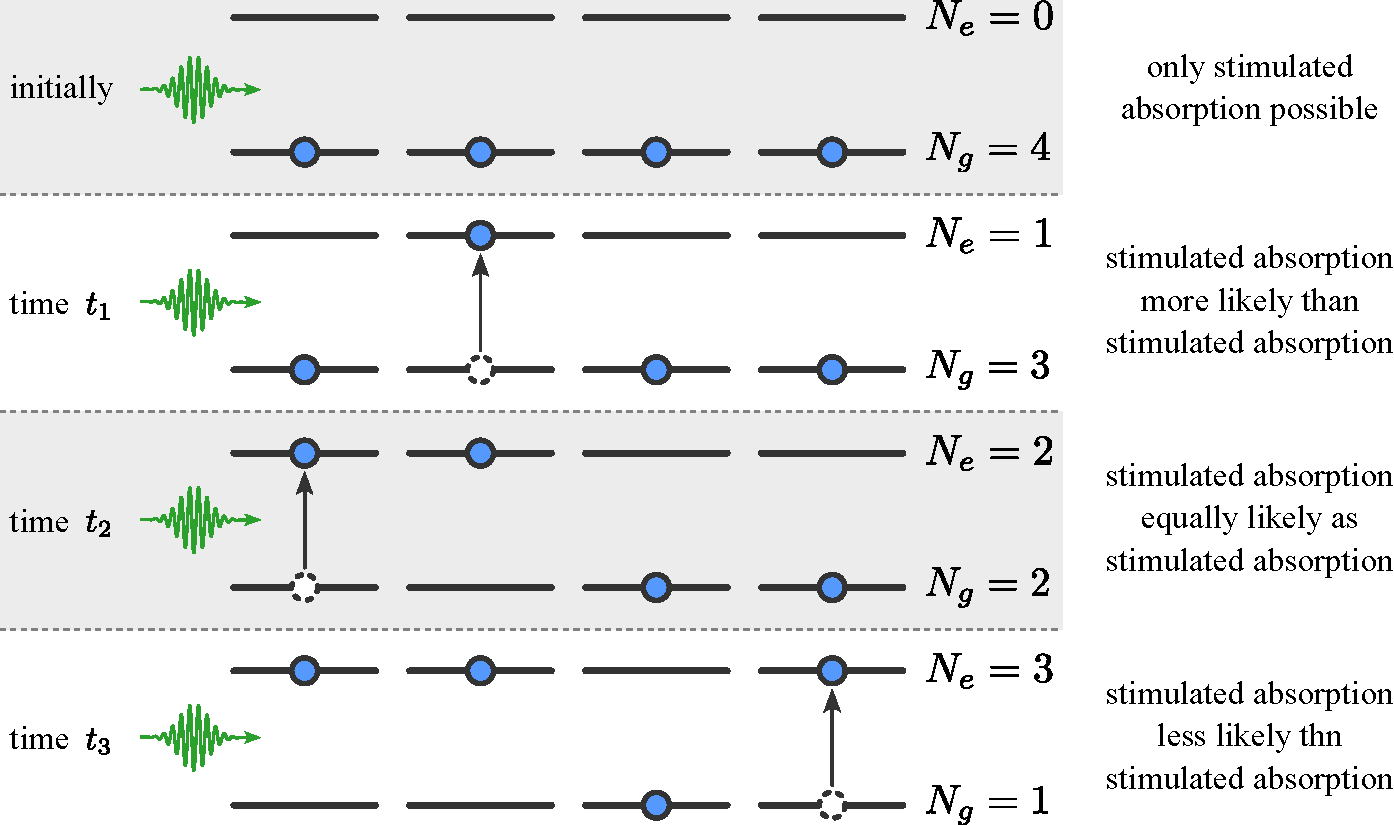
\includegraphics[width=\textwidth]{lesson5/5-3_population_inversion.pdf}
    \caption[Population inversion]{Stimulated emission becomes likely only when most of the atoms are found in the excited state.}
    \label{fig:5-3_population_inversion}
\end{figure}

Let's now consider multiple atoms to see how the situation changes.
Figure~\ref{fig:5-3_population_inversion} depicts four two level atoms.
The probability of spontaneous absorption taking place is proportional to the number of atoms in the ground state, $N_g$.
Not surprisingly, the probability of stimulated emission is proportional to the number of atoms in the excited state, $N_e$.
All atoms are initially in the ground state, $N_g=4$.
The only interaction that is possible for an incoming photon is to get absorbed by one of the atoms.
At a later time $t_1$ there is a new incoming photon.
This time $N_e=1$ and $N_g=3$, meaning both stimulated absorption and emission are possible.
However, stimulated absorption is more likely because more atoms are in the ground state.
Let's say that the photon is absorbed by one of the atoms in the ground state.
At time $t_2$, when a new photon is incident on our group of atoms, both stimulated absorption and emission are equally likely since $N_e=N_g=2$.
For the sake of this example, let's say that this photon is absorbed as well, bring the totally tally to $N_e=3$ and $N_g=1$.
Finally, when another photon at time $t_3$ comes along, it has higher chance of stimulating an emission from one of the excited atoms.
This example demonstrates that if we want to achieve light amplification, we require
\begin{equation}
    N_e > N_g.
\end{equation}
This condition is known as \textit{\textbf{population inversion}}.

It seems that we now have a way of producing an intense and highly coherent light.
There is however one final obstacle that needs to be overcome.
We have seen in Fig.~\ref{fig:5-3_population_inversion} that if $N_g > N_e$, then the incoming photon is more likely to be absorbed and contribute to the population of the excited state.
On the other hand, when $N_g < N_e$, then the incoming photon is more likely to stimulate an emission from one of the excited atoms, contributing to the population of the atoms in the ground state.
This means that in the long-time limit, the population of atoms approaches an equal distribution where $N_g = N_e$.
This means that population inversion is not possible to be achieved for an ensemble of two-level atoms.



\section{Lasers II: Population inversion}
\label{sec:5-4_lasers2}

\begin{figure}[t]
    \centering
    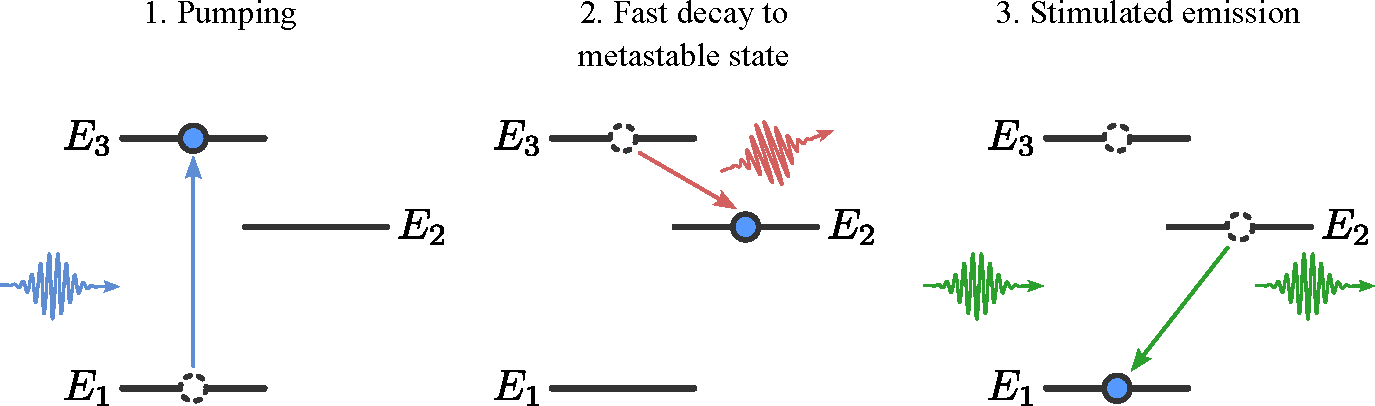
\includegraphics[width=\textwidth]{lesson5/5-4_three-level-atom.pdf}
    \caption[Laser cycle]{Three-stage cycle consisting of pumping via stimulated absorption followed by a quick decay to the middle level via spontaneous emission. The cycle is completed by stimulated emission $E_2 \rightarrow E_1$ contributing to lasing.}
    \label{fig:5-4_three_level_atom}
\end{figure}

We said in the previous section that we cannot achieve population inversion with a simple two-level atom.
Three-level atoms on the other hand are much more suitable for this task as we will learn in this section.
Figure~\ref{fig:5-4_three_level_atom} shows an example of such a three-level atom and demonstrates the basic working principle of a laser.
The ground state is labelled with $E_1$, the middle excited state with $E_2$, and the top excited level with $E_3$.
We assume that the new level $E_3$ is \textit{\textbf{unstable}}, meaning that whenever the atom is excited to level $E_3$, it very quickly decays via spontaneous emission to the middle level $E_2$.
We also assume that level $E_2$ is \textit{\textbf{metastable}}, meaning the atom does not quickly decay to the ground state.

Before addressing the issue of population inversion, let's have a look at the lasing cycle, which consists of the following three stages:
\newline
\textit{\textbf{1. Pumping:}}
We assume that the atom is initially in the ground state $E_1$.
The atom is then pumped to the excited level $E_3$ by a strong pump laser represented by the blue arrow in Fig.~\ref{fig:5-4_three_level_atom}.
Provided that the energy levels $E_2$ and $E_3$ are well separated, the pump laser has small probability of exciting the atom to level $E_2$.
\newline
\textit{\textbf{2. Fast decay:}}
Due to the instability of level $E_3$, the atom quickly decays to the middle level $E_2$ represented by the red arrow in Fig.~\ref{fig:5-4_three_level_atom}.
We have learnt that photons produced via spontaneous emission travel in a random direction.
These photons do not contribute to the amplification of light.
\newline
\textit{\textbf{3. Stimulated emission:}}
Finally, a photon of energy $E_2-E_1$, interacts with the atom causing it to decay to the ground state via stimulated emission.
The transition $E_2\rightarrow E_1$ is known as \textit{\textbf{lasing transition}}.
Photons produced via this transition are the ones contributing to light amplification.

This demonstrates why we need the pump.
Its role is to make sure there are enough atoms in the middle level $E_2$.
Now we see how population inversion can be achieved using three-level atoms.
By using an intense pump, we decrease the population of the ground state $N_1$.
The instability of level $E_3$ and relative stability of $E_2$ ensure that
\begin{equation}
    N_2 > N_1.
\end{equation}

\begin{figure}[t]
    \centering
    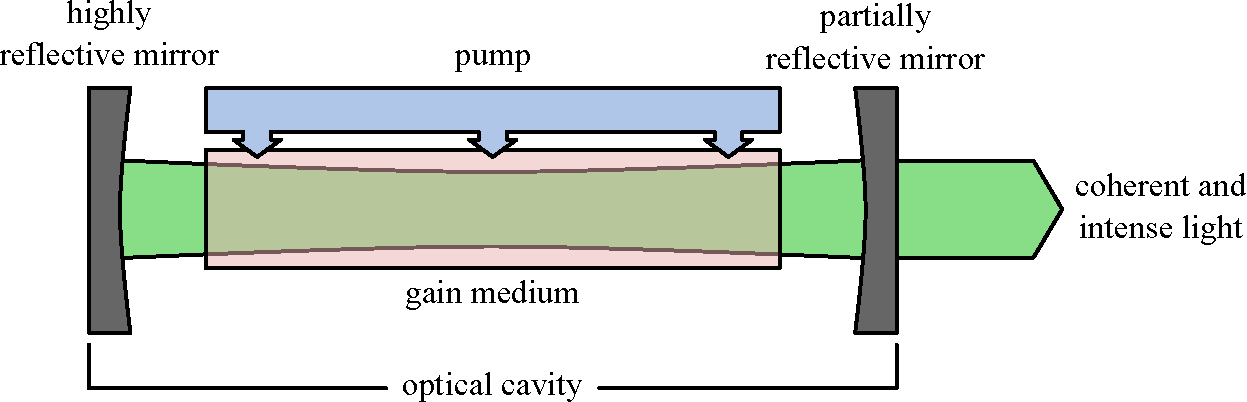
\includegraphics[width=\textwidth]{lesson5/5-4_laser construction.pdf}
    \caption[Laser construction]{Basic construction of a laser.}
    \label{fig:5-4_laser_construction}
\end{figure}

Having described the basic working principle of a laser, let's see what are the main components of a laser.
Figure~\ref{fig:5-4_laser_construction} depicts the basic construction of a laser.
The \textit{\textbf{gain medium}} is the ensemble of our three-level atoms.
Left to their devices, the atoms will mostly be found in the ground state.
Turning on the pump will begin the lasing cycle.
Initially, the excited atoms will decay via transitions $E_3 \rightarrow E_2 \rightarrow E_1$ through spontaneous emission and the produced photons will mostly be incoherent.
Some of the photons emitted from the transition $E_2 \rightarrow E_1$ will be reflected by the mirrors and remain in the \textit{\textbf{optical cavity}}.
These photons will move through the gain medium again where they will encounter a significant population in the middle level $E_2$.
Now the atoms will decay through stimulated emission, producing coherent photons with the ones that were reflected by the mirrors.
Each time the photons get reflected from the mirrors, they stimulate further emission from the lasing transition leading to very intense coherent light inside the optical cavity.
In order to extract this light, one of the mirrors is only partially reflective and a portion of the coherent light is transmitted resulting in an intense and coherent beam of light outside the optical cavity.
Eventually, the number of photons inside the optical cavity reaches a steady state where the rate of production of new photons via stimulated emission balances the rate of loss of photons due to partially reflective mirror.

Having learned about the fundamental working principles and basic construction of the laser, it is time to make our discussion a bit more quantitative.
If the pump is weak, we cannot observe any lasing.
once the rate at which the gain medium is pumped reaches a certain \textit{\textbf{threshold}}, lasing takes place.
In the remainder of this section, we discuss a simplified nonlinear dynamical model that captures this behavior.

The two variables of interest are the number of photons inside the optical cavity, denoted by $n(t)$, and the number of atoms in the state $E_2$, denoted by $N_2(t)$.
We added explicit time dependence $t$ as we are interested how the two variables change in time.
During the lasing process, the number of photons rapidly increases resulting in a large positive rate of change of the number of photons.
\michal{This rate of change is given by the time derivative of the number of photons by $dn(t)/dt$.
Time derivatives are often written with a ``dot'' above the changing variable, $dn(t)/dt = \dot{n}(t)$, which we will use in the rest of this Section as well.}
This rate of change is given by the following difference,
\begin{equation}
    \dot{n}(t) = \text{gain} - \text{loss}.
    \label{eq:5-4_n_dot_basic}
\end{equation}
The gain represents processes that contribute to the number of photons $n(t)$.
In our case, this captures the effect of stimulated emission.
The amount of gain depends on both the number of photons $n(t)$ as well as the population of excited atoms $N_2(t)$.
In the absence of either, the gain vanishes, therefore we can write
\begin{equation}
    \text{gain} = G n (t) N_2(t).
    \label{eq:5-4_gain}
\end{equation}
We have introduce the gain coefficient $G>0$ which captures the strength of the pumping process.
The loss represents photons escaping the optical cavity.
More photons inside the optical cavity lead to larger loss term,
\begin{equation}
    \text{loss} = k n(t),
    \label{eq:5-4_loss}
\end{equation}
where $k>0$ is the loss coefficient.
Substituting Eqs.~(\ref{eq:5-4_gain}) and (\ref{eq:5-4_loss}) into Eq.~(\ref{eq:5-4_n_dot_basic}), we obtain
\begin{equation}
    \dot{n}(t) = G n(t) N_2(t) - k n(t).
    \label{eq:5-4_n_dot_detailed}
\end{equation}

Next, we make the crucial observation that stimulated emission decreases the the population $N_2(t)$.
The more photons present in the optical cavity the more likely that stimulated emission takes place.
Equally importantly, we must realize that in the absence of lasing, the pump maintains a constant population $N_2(t) = N_0$.
This allows us to write the population of excited atoms as
\begin{equation}
    N_2(t) = N_0 - \alpha n(t),
    \label{eq:5-4_population}
\end{equation}
where $\alpha$ is the rate of stimulated emission.
Substituting Eq.~(\ref{eq:5-4_population}) into Eq.~(\ref{eq:5-4_n_dot_detailed}) leads to our final expression for the rate of change of photons inside the optical cavity,
\begin{equation}
    \dot{n}(t) = (G N_0 - k) n(t) - \alpha G n^2(t).
    \label{eq:5-4_n_dot_final}
\end{equation}

\begin{figure}
    \centering
    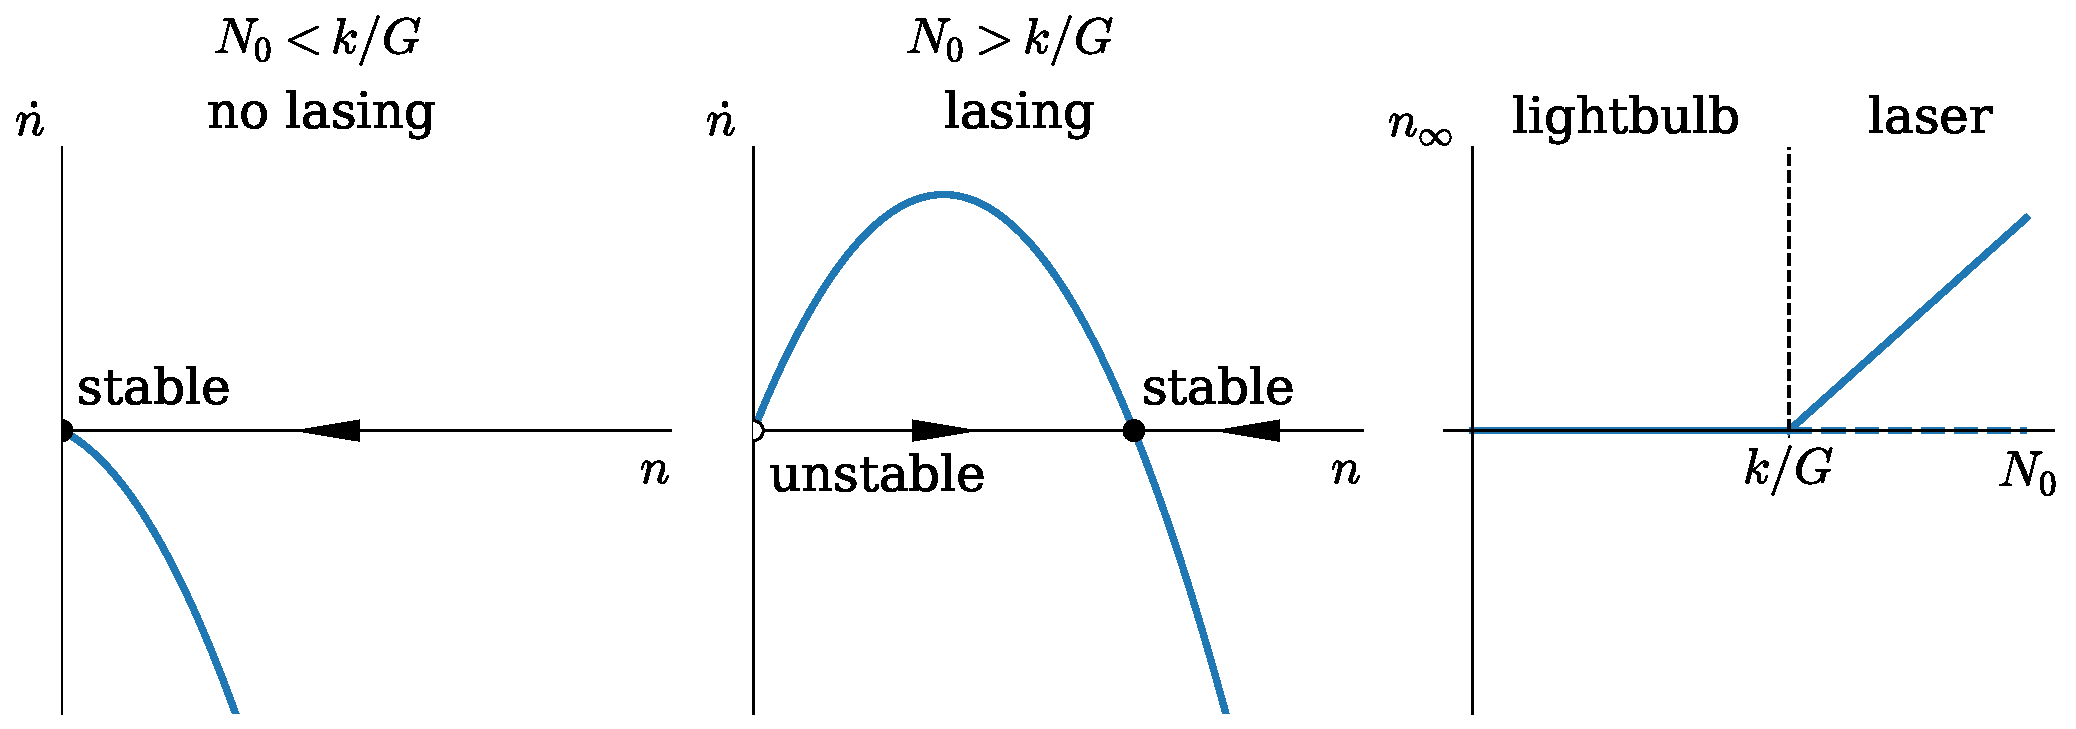
\includegraphics[width=0.9\textwidth]{lesson5/5-4_lasing.pdf}
    \caption[Dynamical model of a laser]{Solutions to the dynamical model of a laser in Eq.~(\ref{eq:5-4_n_dot_final}).}
    \label{fig:5-4_lasing}
\end{figure}

\rdv{maybe use "derivative"? Recheck description of stable point for clarity. Possibly describe as bathtub?}

Eq.~(\ref{eq:5-4_n_dot_final}) is not easily solved analytically.
And frankly, such a solution would not be very enlightening anyway.
To gain better understanding of the dynamics between the number of photons in the optical cavity $n(t)$ and the number of excited atoms $N_2(t)$, we proceed by using graphical methods of analysis.
We are interested in how the rate of change of the photon number $\dot{n}(t)$ changes as a function of $n(t)$ in different parameter regimes.
We observe from Eq.~(\ref{eq:5-4_n_dot_final}) that when the gain is such that $G < k / N_0$, the right-hand-side of the equation is negative, $\dot{n}(t) < 0$, for any $n(t)$ because the number of photons can only be non-negative.
This means that regardless of how many photons we start with, eventually they will all leak from the cavity and $n(t)$ will always tend to zero.
The left panel of Fig.~\ref{fig:5-4_lasing} shows a plot of $\dot{n}(t)$ versus $n(t)$ in this weak-gain regime.
We see that the rate of change of the photon number is indeed negative as predicted.
The arrow on the horizontal axis represents the flow of $n(t)$ as time progresses.
It always decreases and asymptotically approaches the stable \textit{\textbf{fixed point}} $n_{\infty} = 0$, where $\dot{n}(t) = 0$.
There is no lasing when we are in this weak-gain regime.

Now let's look at the strong-gain regime when $G > k / N_0$.
In this case, the right-hand-side of Eq.~(\ref{eq:5-4_n_dot_final}) may be positive as well as negative.
This means that for some starting values of $n(t)$ the photon number will decrease.
But for some starting values, $n(t)$ will increase as lasing will take place.
The middle panel of Fig.~\ref{fig:5-4_lasing} depicts this regime.
This time, $\dot{n}(t) = 0$ has two solutions and therefore there are two fixed points.
One of them is our old fixed point $n_{\infty} = 0$.
Unlike before, this fixed point is now unstable, meaning that any small deviation from it will result in further increase of $n(t)$ which will flow towards a new stable fixed point at a finite value.
The unstable fixed point is represented by an empty circle in Fig.~\ref{fig:5-4_lasing} while the stable fixed point is solid.
We can observe amplification of the photon number which is a clear sign of lasing.

The last panel on the right of Fig.~\ref{fig:5-4_lasing} summarizes our analysis of Eq.~(\ref{eq:5-4_n_dot_final}) by plotting the fixed points $n_{\infty}$ and their stability.
When $G < k / N_0$, there is only a single fixed point at $n_{\infty} = 0$.
In this regime the atoms are weakly pumped and decay via spontaneous emission producing incoherent light, just like a light bulb.
When $G > k / N_0$, two fixed points exist.
The stable fixed point is represented by the solid line, while the unstable one is represented by the dashed line.
It is in this regime where lasing takes place.


\section{Single photons}
\label{sec:5-5_single_photons}

Lasers are excellent sources of intense coherent light and are indispensable in modern fiber-optic communication.
Pulses of laser light can be used to encode classical bits.
Presence of a pulse can encode a 1 and absence of a pulse can encode a 0.
Such encoding has a number of desired properties making it suitable for classical communication.
It is robust against \textit{\textbf{attenuation}}.
Due to the large number of photons constituting a single pulse, loss of a few of them along the fiber presents no issue, and the message remains legible to a decoder at the destination.
Even if the pulse travels a large distance along the fiber and attenuation becomes a problem, the message can be read and \textit{\textbf{amplified}} along the way.
Finally, producing these pulses of light is relatively easy and therefore \textit{\textbf{reliable}}.

On the other hand, intense pulses of laser light cannot be put in a quantum superposition and they cannot be entangled with other systems.
This makes the above encoding scheme entirely unsuitable for quantum communication.
In order to exploit the full toolbox of quantum mechanics, we have to use single photons.
In this section, we outline the three basic methods of producing single photons.

\begin{figure}
    \centering
    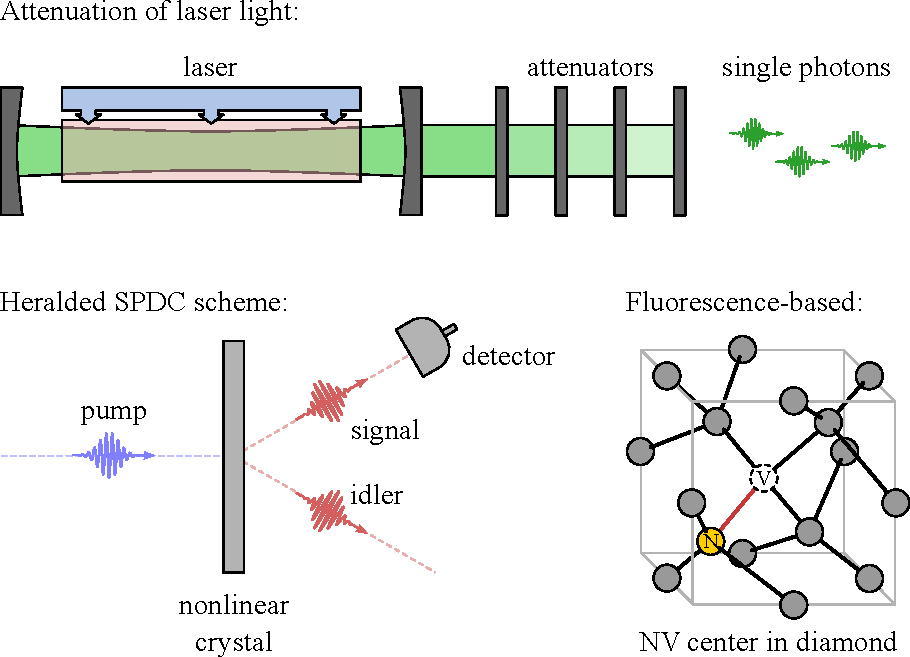
\includegraphics[width=0.9\textwidth]{lesson5/5-5_single_photons.pdf}
    \caption[Single photon sources]{Different approaches to creating single photons.}
    \label{fig:5-5_single_photons}
\end{figure}

The first method relies on gradual \textit{\textbf{attenuation of laser light}} as shown in
the top panel of Fig.~\ref{fig:5-5_single_photons}.
The intense laser pulse exiting the optical cavity is passed through a series of attenuator plates.
Each plate transmits only a portion of the laser light and therefore decreases the pulses intensity.
This process is repeated until the average energy of the pulse, $\lambda$, is less than that of a single photon.

This approach to producing single photons is conceptually simple but suffers from a number of serious issues.
Firstly, this source of single photons is probabilistic.
The number of photons contained in the pulse after the attenuation process follows a Poissonian distribution.
If the average number of photons per pulse is $\lambda = 0.1$, then the probability of there being zero photons is 90.5\%, probability of a single photon is 9.1\%, and probability of two photons is 0.4\%.
Most of the time, the pulse becomes completely attenuated and the process of generation of single photons fails.
There is also a finite probability that this method generates more than one photon, which is highly undesirable in quantum communication.

The second issue is quite technical but very important, and has to do with something called the \textit{\textbf{second-order correlation function}} $g^{(2)}(\tau)$.
The full derivation of this function is well beyond the scope of this book but its meaning is not so complicated.
The second-order correlation function $g^{(2)}(\tau)$ tells us how likely it is to detect two photons, one at time $t$, and the other one at time $t+\tau$.
Particular case of interest in our discussion is when the time interval between the detection events vanishes, $\tau = 0$.
For ideal single photons the second-order correlation function $g^{(2)}(0) = 0$.
This is quite intuitive since we should not detect the same photon twice.
We say that a single-photon source produces light which is \textit{\textbf{anti-bunched}}.
For realistic sources, as long as $g^{(2)}(0) < 1$, we say the light is anti-bunched and possesses quantum properties.
On the other hand, for classical light $g^{(2)}(0) \geq 1$, and when it is strictly larger than unity, we say the light is \textit{\textbf{bunched}}.
Laser light is neither bunched nor anti-bunched as $g^{(2)}(0)=1$.
Since the single photons produced by attenuation started as a laser they are not anti-bunched.
This is a problem because numerous protocols in quantum computation require anti-bunched light.

The second method of producing single photons is via \textit{\textbf{heralded spontaneous parametric down-conversion}} shown in the lower left panel of Fig.~\ref{fig:5-5_single_photons}.
We have discussed the basics of SPDC in Section~\ref{sec:4-4_spdc} where we used it to produce entangled pairs of photons.
Conversion of a single high energy photon into two photons of lower energy can be also used as a source of single photons by using the fact that the two produced photons have a well-defined direction of travel.
We can detect one of these photons in order to herald presence of a single photon in the other mode.
The high-energy photon is sometimes called the \textit{\textbf{pump}}, the low-energy photon that gets detected is the \textit{\textbf{signal}}, and the heralded photon is the \textit{\textbf{idler}}.
This scheme is still probabilistic as the SPDC is a very rare process meaning we have to try many times before we produce a heralded single photon.
In some cases this rarity can be an advantage because once we detect the signal photon we have a very high probability that the idler mode contains only a single photon.
The properties of the detector also affect this scheme.
Real detectors are not 100\% efficient, meaning sometimes a signal photon goes undetected.
This might be annoying but really it just means that we have to try the whole process again.
More importantly, real detectors have a finite \textit{\textbf{dark count rate}}, meaning occasionally they register a detection event even in the absence of a signal photon.
This ``heralds'' a non-existent idler photon and has a deleterious effect on any quantum communication protocol relying on single photons produced by this scheme.

The last approach to producing single photons is through \textit{\textbf{fluorescence}} of atoms and molecules.
The idea is basically the same as the one we have been discussing throughout this Chapter.
A physical system with discrete levels is first excited to a higher energy level and later transitions back to a lower energy level by emitting a single photon.
However, the two- and three-level systems we have been using so far are simplifications of real physical systems.
One promising source of single photons that is currently under intense research focus are \textit{\textbf{nitrogen-vacancy centers in diamond}}, shown in the lower right panel of Fig.~\ref{fig:5-5_single_photons}.
The NV center consists of a nitrogen atom $N$ located next to a vacant site $V$ of a diamond lattice.
This vacancy is used to trap an electron whose \emph{spin}\index{spin} then acts as a qubit~\footnote{You should have already studied the basics of atomic structure, but for the record, electrons generally have two states that can be described as "spin up" and "spin down", which we write as \ket{\uparrow} and \ket{\downarrow}}.
The electron qubit can be manipulated optically, can retain its quantum properties even at room temperatures, and acts as an excellent source of single photons with nearly vanishing second-order correlation function $g^{(2)}(0)$.
All these properties make NV centers in diamond very promising physical systems for quantum communication.


\newpage
\begin{exercises}
\exer{Consider the following quantum state:}
\begin{equation*}
\ket{\psi} = \frac{\sqrt{3}}{2}\ket{0} + \frac{1}{2}\ket{1}
\end{equation*}
\subexer{Find the probability of measuring a zero.}
\subexer{Find the probability of measuring a one.}


\end{exercises}

